\begin{acronym}
\acro{evm}[EVM]{Ethereum virtual machine}
\acro{eoa}[EOA]{externally owned account}
\acro{utxo}[UTXO]{unspent transaction output}
\acro{dapp}[DApp]{decentralized application}
\acro{ipfs}[IPFS]{Interplanetary File System}
\acro{ico}[ICO]{initial coin offering}
\acro{erc}[ERC]{Ethereum request for comment}
\acro{api}[API]{application programming interface}
\acro{pow}[PoW]{proof of work}
\acro{pos}[PoS]{proof of stake}
\acro{asic}[ASIC]{application-specific integrated circuit}
\end{acronym}

\section{Introduction}
Software continuously changes the way we communicate, work, learn, play
and almost every other aspect of our lives.
Progress, however, rarely comes without new drawbacks.
One of the drawbacks of our more and more digital lifestyle is that we give an ever increasing amount
of control into the hands of large institutions and corporations.

The ways in which this might hurt us are numerous. Google has the
power to single-handedly remove inconvenient sites from their search index, thereby
practically removing them from the internet for a large part of
the population. There are several cases where news distributors
have been brought down and made unreachable by cyber attacks. It is
easy to imagine non-democratic governments manipulating the results
of elections to their liking. Banks and insurance companies
increasingly base their decisions on the outputs of closed machine learning
systems which only few people understand.

What if we could give these systems back into the hands of the people they
influence the most, allowing them to understand exactly how they work and
making sure that no single party can manipulate them in unwanted ways?


This is the promise of \emph{Ethereum} and \emph{smart contracts}.
The present report explores how to work with this technology
given a simple example explained in the next section.

% TODO add some citations

\section{Smart Tipping for Tutor Groups}
\label{sec:demo}
In this section we describe a not completely serious but educative
use case from the university context. At heart it is a performance-based
remuneration contract, which could be converted to a financial
derivative or insurance with minimal context changes.

University courses are typically broken down into lecture and
exercise units. The exercises are an essential part in the student's
venture of achieving a good grade and are handed off to
PhD students besides their actual work without getting enough extra time allocated.

A typical approach to motivate and gratify the tutor in such
a situation would be monetary, e.g. by tipping.
This however leaves us with the question when the tips will be payed.

In a first option, students tip the tutor at the beginning of the semester.
This forces the students to trust the tutor with doing a good
job despite already having received his incentive.

In a second option, students tip the tutor at the end of the semester.
Now the tutor has to trust the students to actually tip him despite already having received the service.

This is a common situation where both parties do not necessarily know and therefore trust each other upfront.
It makes it difficult to agree on a way of conducting a transaction.

Is there a solution which does not require mutual trust?
Imagine a third party, which accepts the tips of the students
at the beginning of the semester and tells the tutor how much he
would get if he does a good job. But only if the results are
satisfactory he is payed out, otherwise the tips are
returned to the students.

Both the students and the tutor now only have to trust this
third party and not each other.
Smart Contracts can be used to build such a third party, and one that is easy to trust on top,
since they are deterministic and immutable computer programs with their source code publicly available to everyone.

% TODO add concept chart of smart contract

\section{Ethereum}

Blockchain technology has several important strengths:

\begin{itemize}
\item {\em Decentralization} creates natural resistance against
  data loss e.g. through natural disasters or hacker attacks.
\item {\em Trustlessness} facilitates transactions between parties that
  do not know each other.
\item {\em Immutability} prevents data from being manipulated by individual
  parties.
\item {\em Publicness} makes the data available to all participants and
  can counteract it from accumulating in corporations and institutions.
\end{itemize}

Bitcoin introduced the blockchain technology and its advantages for
monetary transactions, but it is easy to see that these attributes
are interesting for a much wider range of applications.
In 2014, Vitalik Buterin wrote the first version of the Ethereum
Whitepaper \cite{Buterin14}, a new type of blockchain on top of which
general programs can be build.
The native currency is called \emph{Ether (ETH)}. 

One way to describe Ethereum is as a ``world computer'', which is
not owned by a single entity and is not located at a single place,
but is constituted and shared by everyone who participates in it.
The programs developed for this computer are called \emph{smart contracts} and run in a simple, stack-based virtual
machine, the \ac{evm} \nocite{Saini18}.
The \ac{evm} is defined in the {\em Yellow Paper} \cite{Wood18}, which is mainly maintained by Dr. Gavin Wood.

The deployment model is given by contract accounts.
Ethereum has two types of accounts (cf. \cite{Kenneth18}]):

\begin{enumerate}
\item {\em \acp{eoa}} belong to a person and are controlled by a private key.
\item {\em contract accounts} have a public address and an Ether balance like
  \acp{eoa}, but instead of a private key, they are controlled by the associated smart contract.
\end{enumerate}

\subsection{Technicalities}

\subsubsection{Consensus}
Ethereum uses a \ac{pow} algorithm called \emph{Ethash} at the time of this writing.
It is based on the Keccak hash function.
Ethash is designed to be memory-intensive, thereby making it hard to develop \acp{asic} for mining.
This aims at counteracting the concentration of mining power in pools of large and financially-strong entities
that can afford such specialized hardware (cf. \cite{Buterin2013}).

\subsubsection{State Storage}

\begin{figure}[]
	\centering
	\includegraphics[width=0.8\linewidth]{"resources/blocks".png}
	\caption{Ethereum Blocks}
	\label{fig:blocks}
	Two blocks from the Ethereum blockchain.
	The state trees are expanded and how the updated value of account 175
	is persisted using copy-on-write technique.
	Image taken from \cite{Buterin2015}.
\end{figure}

Ethereum can be seen as a state machine.
Every transaction changes it from one state to a new state.
In contrast to Bitcoin, state is represented on account level rather than
transaction level.
Technically, Ethereum stores all state in a data structure called \emph{Merkle-Patricia tree} \cite[sec.~4.1]{Wood18}.
It can be used to efficiently validate the integrity of blocks (Merkle tree)
as well as for efficiently querying elements (Patricia tree).
The tree nodes are indexed by their hashes and persisted in a key-value-store.

Each block consists out of three such trees: one for transactions, one for transaction receipts and one for the state \cite{Buterin2015}.
The tree structure also provides an efficient copy-on-write mechanism for changing data (cf. Figure~\ref{fig:blocks}).

\subsection{Gas}

Code associated with a blockchain transaction has to be executed by every miner validating a block.
Bitcoin allows users to write their own transaction validation scripts,
but the language is not Turing complete and severely limited for security reasons (cf. \cite{Costill16}).
E.g there are no looping constructs to stop users from writing infinite loops.
A blockchain with a general programming model needs a concept to keep resource usage under control.

Ethereum's solution to this problem is called {\em gas}. In Ethereum,
every instruction the \ac{evm} has to execute and every byte that has
to be stored in the blockchain consumes a defined amount of gas (cf. \cite{Rosic18}).
Whenever someone initiates a transaction, he decides upon two parameters:

\begin{itemize}
\item The \emph{gas price} denotes how much Ether the initiator is willing
  to pay for each consumed unit of gas.
  
\item The \emph{max gas} value denotes how much gas the transaction may
  consume in total.
\end{itemize}

Miners select transactions to include in their blocks based on these parameters,
thereby making resource usage on Ethereum a self-contained market where prices can change
in relation to real-world operating expenses, e.g. improving computing hardware or power pricing (cf. \cite{Aggarwal17}).

While the transaction executes, the allotted gas amount (max gas) is incrementally consumed.
If the transaction completes before the gas is used up, the remaining gas is returned
to the initiator. If the gas runs out before the transaction completes, it is aborted
and all changes are reverted (the miner still receives the used gas). 

\subsection{Decentralized Applications}

The terms \emph{smart contract} and \emph{\ac{dapp}} are frequently encountered when working with
blockchains like Ethereum.
A \ac{dapp} typically describes a classical web application where the
centralized backend (e.g. a MySQL database) has been replaced by a stack of decentralized
smart contracts.
There are ventures to decentralize the frontend as well (e.g. the  \ac{ipfs}~\cite{Benet14}),
but these are not commonly used as of today and we will not talk more about them in this report.

\subsection{Common Use Cases}

While smart contracts can be arbitrary programs,
some use cases fit the blockchain technology especially well.
We introduce some of these below.

\subsubsection{Stake/Ownership Management}

Probably the oldest and most widely known use case for smart contracts is managing
stake or ownership in some underlying asset, e.g. a company or real estate.
We call these systems \emph{token systems}. The basic idea is the following: We implement a smart
contract that acts as a proxy for this asset and spread the total value out across
a specified amount of tokens. Users can then transfer currency to this contract and
in return receive tokens which certify their stake in the asset.
This is the underlying mechanism of \acp{ico} which have received some attention in recent times.
The use case is so common that multiple standard interfaces for token contracts have been defined:
\acs{erc}20~\cite{Vogelsteller15} and \acs{erc}721~\cite{Entriken18}.

\subsubsection{Financial Services/Derivatives}

This class includes insurance contracts, speculative financial products and performance
based remuneration systems amongst others.
The example introduced in Section~\ref{sec:demo} also belongs
to this category.
The abstract idea is having a pot into which multiple parties pay in
currency.
Then it gets decided based on external events who receives back how much of the
total volume.

\subsubsection{Unalterable Information Storage}

The blockchain is a natural option when information shall be stored such that it
is publicly available and tamper-proof.
Examples could be scientific data or money flows of charity organizations.
Even if the original data must not be publicly available (identity documents, grade reports, health records, \ldots),
the blockchain can still be used to ensure the absence of tampering by storing fingerprints/hashes (cf.\ \cite{Marx18-2}).

\subsubsection{Decentralized Organization}

Smart contracts can be used to make decisions in large, distributed groups where
members do not necessarily know and trust each other. One early example of this is
DASH, a cryptocurrency that makes use of itself to coordinate its development process
(cf.\ \cite{Galt2015}). This technology could e.g. allow for tamper-proof elections
in countries with incredible and corrupt governments.

\section{Writing Smart Contracts}

In this section, we talk about the development of smart contracts in context
of developing the example introduced in section~\ref{sec:demo}.

\subsection{Smart Tipping System}

\begin{figure}[]
	\centering
	\includegraphics[width=\linewidth]{"resources/Smart Tipping Design".pdf}
	\caption{Design of the Smart Tipping System}
	\label{fig:smarttipper}
\end{figure}

The smart tipping system comprises two contracts (cf. Figure~\ref{fig:smarttipper}).
The simpler one is an oracle contract used by university employees to write
grade reports into the blockchain.
We talk more about this necessity in Section~\ref{sec:dev:isolation}.
The second one is the actual tipping contract.
The workflow is as follows.
\begin{enumerate}
	\item Either party creates an instance of a tipping contract at the beginning of the semester.
		At this point, both parties decide on a target grade
		determining if the tutoring will be considered successful.
	\item The students pay in their tips. Both parties can check the current volume of the contract at any time.
	\item At the end of the semester, either party triggers the resolution of the contract.
	\item The tipping contract checks the grade results published by the university.
		If it is better than the defined threshold, the tutor is payed out the accumulated tips.
		If it is not satisfactory, the money is payed back to the students.
\end{enumerate}

\subsection{Development Process}

The \ac{evm} defines its own byte-code to which smart contracts are compiled.
There are several high-level languages to develop smart contracts,
the most common one is \emph{Solidity}~\cite{Solidity}. 

The high-level process of developing a \ac{dapp} involves following steps:

\begin{enumerate}
    \item Developing the smart contract code.
    \item Compiling the smart contract code in order to obtain deployable byte-code and interface
        specifications that can be used from the frontend.
    \item Deploying the contract code to the blockchain.
    \item Writing and deploying the frontend code.
\end{enumerate}

Most \ac{dapp} developers use the \emph{Truffle Framework}~\cite{Truffle} at the time of this writing.
It provides tools such as

\begin{itemize}
    \item Solidity compiler,
    \item scriptable contract deployment framework,
    \item unit testing framework,
    \item test chain for local testing ("Ganache") and
    \item libraries simplifying the integration of smart contracts with frontend code ("Drizzle", "web3").
\end{itemize}

This report focuses on the development of smart contracts.
For the other steps of the development process, the homepage of the Truffle framework is a good starting point.

\subsection{Solidity}

Solidity is a language with strong influences from JavaScript and C++.
The concept of classes has been rebranded as contracts,
but conceptually they are similar. We can create instances of contracts and deploy them
to the blockchain. A contract can have member variables and methods, methods in turn can
have local variables.
Listing~\ref{listing:oracle} shows the simple oracle contract from our example use case.

\begin{listing}[]
\inputminted[breaklines,fontsize=\footnotesize]{solidity}{TUMOracle.sol}
\caption{Grade Oracle Contract}
\label{listing:oracle}
\end{listing}

\subsubsection{Storage}

Solidity provides simple types like integers and complex types like structs, arrays and
hashmaps (which are called mappings). Noteworthy are the absence of floating point numbers
(fixed point numbers are in development but not yet supported at the time of this writing, cf.\ \cite{SolidityTypes}).
Integer size can be defined very granuarly from 8bits to 256bits in 8bit steps.
This is important because each stored byte has costs gas.

The \ac{evm} has two types of memory: \emph{local memory} and \emph{contract storage}.
Local memory is volatile and supports the execution of smart contract methods. It uses
a stack for function arguments and linearly addressable memory for local variables.
Contract storage is persistent and part of the contract account. Conceptually
it can be thought of as a 256bit-addressable byte array, but it is implemented as a key-value-store
to account for how sparsely\footnote{A 256bit-addressable byte array can hold more than $10^{68}\mathrm{GB}$.}
this array will be populated (cf.\ \cite{Marx18}).

\subsubsection{Error Handling}

The \ac{evm} has two error modes: \emph{expected errors} and \emph{unexpected errors} (cf.\ \cite{Maurelian17}).

Expected errors are caused by failing parameter validations (\texttt{require()} function) and by explicit calls to \texttt{revert()}.
When an expected error happens, all changes are
reverted and the {\em remaining gas is returned to the transaction initiator}.

Unexpected errors are caused by failing \texttt{assert()} calls, array access with negative
index, etc.
In this case, changes to the chain are reverted and {\em all remaining gas is used up}.

It is good practice to check user inputs wherever possible using \texttt{require()} statements. 

\subsubsection{Isolation}
\label{sec:dev:isolation}

The reader might wonder why the presented system uses a separate grade oracle contract
instead of directly accessing already existing interfaces of the university.
It turns out that this is not possible.
Every execution of contract code must be executed by different miners on different
computers every time the containing block is validated.
The execution must deterministically yield the same result,
otherwise reaching consensus about the validity of transactions would not be possible.

This has two practical implications:

\begin{itemize}
    \item The \ac{evm} provides no mechanisms for randomness.
    \item There is no access to external systems. Contracts can only work with data stored in the blockchain.
\end{itemize}

The second point creates the need for so-called \emph{oracle accounts}.
These are simple smart contracts that proxy institutions and serve as a gateway to get
external data into the blockchain (cf.\ \cite{Gall18}).

\subsubsection{Inter-Contract Communication}

To create more complex systems (e.g. using data from oracle contracts),
contract methods must be able to call other contract methods.
To do so, two things are necessary:
Firstly, the code of the callee contract is needed by the Solidity compiler in order to properly compile and link the call.
Secondly, the address of the deployed instance of the callee contract must be known so that calls can be forwarded.
Given these two things, a proxy object for the instance can be instantiated and used like a local object.
Typically the address of the callee is provided as constructor parameter.
Listing~\ref{listing:oracle} outlines this process using the relevant parts of the smart tipping contract.

\begin{listing}[]
\inputminted[breaklines,fontsize=\footnotesize]{solidity}{intercontract.sol}
\caption{Inter-Contract Calls}
\label{listing:oracle}
\end{listing}

\subsubsection{Reads and Writes}

Calls to smart contracts can either be read-only operations or modify the state of the blockchain.
Read operations do not trigger a transaction, are executed synchronously and do not consume gas (cf.\ \cite{Hitchens18}).

Write operations trigger transactions and do consume gas.
Two things are important when working with transactions:
Firstly, writes to the blockchain are not only triggered by explicit assignments to the contract storage but also when events
are emitted (cf. Section~\ref{sec:dev:events}).
Secondly, transactions are executed asynchronously
since they have to be mined to become valid. As one result, calling a
write operation does not return a value but a \emph{transaction receipt}~\cite[sec. 4]{Wood18}.
At the time of this writing, Solidity however allows defining return values for
write operations and the compiler does not catch when they are used.
This is a common source of confusion amongst new Solidity developers.

\subsubsection{Events}
\label{sec:dev:events}

\begin{listing}[]
\inputminted[breaklines,fontsize=\footnotesize]{solidity}{Event.sol}
\caption{Emission of Events}
\label{listing:events-emit}
\end{listing}

\begin{listing}[]
\inputminted[breaklines,fontsize=\footnotesize]{javascript}{Event_ui.js}
\caption{Event Handling Using the Web3 Library}
\label{listing:events-subscribe}
\end{listing}

Since transactions are executed asynchronously, we need an asynchronous mechanism
to communicate their results and effects to other systems.
Solidity provides such a mechanism by the means of \emph{events}~\cite{ConsenSys16}, which make use of the underlying Ethereum
logs~\cite[sec. 4]{Wood18}. Solidity code can define and emit structured events,
which client libraries can subscribe and react to using the publish/subscribe paradigm. % TODO cite something for pubsub
Listings~\ref{listing:events-emit} and \ref{listing:events-subscribe} show how this mechanism
can be used to notify a tutor about new tips.

% \subsubsection{Arrays}

% A notable byproduct of the key-value-store paradigm of Ethereum blockchain storage is the
% absense of array structures % COME BACK TO THIS AFTER RESEARCHING MORE OF THE CURRENT STATE
% https://github.com/ethereum/solidity/issues/2948
% dynamic arrays were allowed in storage..? originally could not return nested arrays such
% as strings and structs, but now it has recently been added as per 2948?

\subsection{Ethereum Development Considerations}

\subsubsection{Compilation and Debugging}Development in the Ethereum ecospace is still in its infant stages. New iterations of the
solidity compiler and companion tools such as the \emph{Truffle Framework} are regularly being
released.

To ensure that contracts behave as expected it is important to add a pragma statement, e.g. '\texttt{pragma solidity \^0.4.18;}', at the
beginning of solidity files which defines the compiler release the code conforms to.

The solidity compiler's error handling tends to lack meaningful and descriptive messages. It can
take patience and thoughtful code review in order to track down difficult syntactic or run-time
errors. This is likely due to the high frequency of releases and hopefully improvements will come
in time.

The current Truffle toolset includes a solidity runtime debugger but the functionality is extremely
limited to what is standard in more mature languages. One noticeable limitation is the
inability to view individual variable states in local memory. At this time, the best method
for tracking variables remains console log statements or emitting events as described in the
previous section.

\subsubsection{Building UIs}The "Drizzle" frontend integration tools are a fast way to quickly build UI interactions with
contracts. There are two flavors, Drizzle-React and Drizzle-React-Components that build on top
of the Ethereum web3 framework in the sequence \emph{Web3 -> Drizzle-React -> Drizzle-React-Components}.
Although the Components are plug and play React elements, they suffer from severe limitations such as the
inability to assign transaction values to messages. With this in mind, it is often the case that
developers will have to go deeper towards web3 in the tech stack until they obtain the
granularity needed for the contract's use case. Another tip is to keep an eye on current
API definitions as recently there have been changes between version releases.

\subsubsection{Testing Contracts}Because deploying contracts to the main Ethereum chain costs gas and suffers from validation delay
it is advisable to use a local test-chain such as Ganache or that included in the Truffle Console.
This drastically speeds up development time, however, most modern browsers use the Metamask wallet
management extension and in its current state it does not work well with local test-chains. The connection
and management of multiple accounts is clunky and cumbersome and can slow down progress.\\[0.2em]

Finally, it is important to realize that documentation and sources of reference regarding \ac{dapp}
development is widely available but often out-dated. A tutorial or resource may be correct for an
outdated pragma/compiler release, but inefficient or broken in current releases. Adding to the confusion
is the multitude of higher-level tools and frameworks which often have different approaches to the same
task. It is advisable to refer to multiple sources and evaluate the merits and suitability of the procedure
before diving in and committing significant development time.


\section{Challenges in Dapp Development}

This section will discuss particular challenges as they apply to both \ac{dapp} 
development on Ethereum, and blockchains in the broader context.

\subsection{Dangers of Immutability}

Along with all the benefits of immutable ledgers, one of the foremost disadvantages
is an inability to modify existing code logic. Once a contract is deployed, it
is incapable of having patches or bug-fixes applied to it. The only manner in which
contract behavior can be modified is to deploy a new contract and have all actors
redirect calls to the address of the new contract. Furthermore, whatever interfaces
remain public and active on the previous contract will still be accessible, as well
as any unintended side effects or transactions which were confirmed via the flawed
code.

An important case study regarding the dangers of flawed contract code
being migrated onto the main Ethereum chain is that of the DAO hack. \cite{DaoHack}

The DAO was a successful crowdfunding initiative launched via token sale which took place
in May of 2016. The premise was to create a trustless and autonomous venture capital
platform where stakeholders could vote on investment opportunities and have fund
allocations and management functions executed solely by Ethereum contract interactions.

A major vulnerability concerning the handling of recursive calls allowed a user to
siphon off 3.6 million Ether of the DAO holdings (around a third of the total value).
The fiat value of Ether at the time of the attack put the stolen amount at approximately
50 million USD.

As alluded to at the beginning of this section, from a technical standpoint, there
is no remedy within the parameters of Ethereum's intended operation. However, given
the gravity of the situation, during a 28 day holding period coded into the original
contract, community leaders contemplated external and oligopolistic methods to
artificially change the state of the blockchain. The two main ways of doing this
are a soft-fork and hard-fork. In the soft-fork scenario, DAO transactions would be
blacklisted going forward. In the hard-fork, the DAO transactions would be reverted and
a parallel chain (fork), through consensus and political influence, would become the
"new" Ethereum going forward. \cite{HardForkSoftFork} In the end, a hard-fork was
executed and this split the community between those who felt it was in the social
interest to interfere externally with the immutability of the Ethereum chain, and
those that felt the blockchain was intended to be a departure from such governing
interferences. The abandoned fork still operates today as an independent entity under
the moniker of Ethereum-Classic, alongside the main Ethereum. \cite{EthereumClassic}

\subsection{Speed and Scalability}

In today's atmosphere of cloud computing, distributed systems, and large scale
infrastructure investment; critical bottlenecks in speed and scalability are often
addressed further along the development process for many applications. However, due to
the need for validation and replication of blocks by miners, transaction time and number
of op-code executions becomes a crucial consideration from the onset of design in blockchain
applications.

\begin{figure}[]
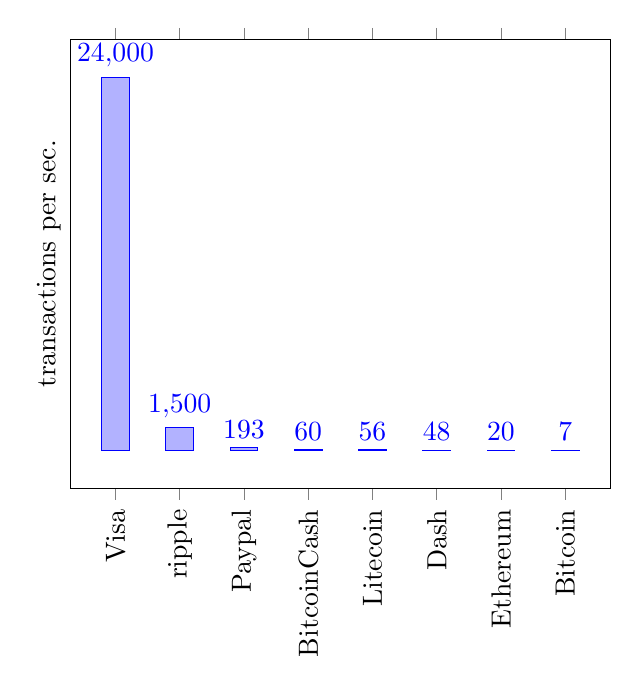
\begin{tikzpicture}
    \begin{axis}[
        ybar, axis on top,
        ytick=\empty,
        %enlargelimits=0.15,
        ylabel={transactions per sec.},
        ylabel near ticks,
        symbolic x coords={Visa,ripple,Paypal,BitcoinCash,Litecoin,Dash,Ethereum,Bitcoin},
        xtick=data,
        xticklabel style={rotate=90},
        nodes near coords,
        %nodes near coords align={vertical},
        ]
\addplot coordinates {(Visa,24000) (ripple,1500) (Paypal,193) (BitcoinCash,60) (Litecoin,56) 
        (Dash,48) (Ethereum,20) (Bitcoin,7)};
\end{axis}
\end{tikzpicture}
\caption{Transactions Speed of Digital Currencies\cite{TransactionSpeed}}
\label{fig:transactionSpeedBar}
\end{figure}

As seen in figure~\ref{fig:transactionSpeedBar}, Ethereum in its current state has an extremely
low transaction throughput. Although the figure compares digital currency transactions, the
mechanisms for \ac{dapp} confirmations is the same. The throughput issue can often be
even more crippling during high loading times such as during an ICO or token launch.

With the scaling and speed limitations in mind, \ac{dapp} development currently favors systems
developed with a hybrid approach of handling non-pertinent transactions and procedures off chain, while
committing stake and value transactions to Ethereum storage. An example of this paradigm
would be CryptoKitties, which stores ownership and DNA (a seed which identifies a unique permutation) on
the blockchain but hosts all digital assets on a centralized server. When the DNA is combined
with the centralized data it generates the user's unique kitty.\cite{CryptoKitties}

\subsubsection{Other Solutions to Scalability and Throughput}

Although developers have found ways to mitigate scalability issues through careful program
design, there is an ongoing push to improve the underlying capabilities of the Ethereum network
and increase transaction speed through incremental changes to the underlying technology. In the
Ethereum sphere there are two such solutions which are gaining heavy support. First is shifting
the consensus method from \acf{pow} to \acf{pos} and the other is sharding
and side-chaining.

Ethereum is currently using \ac{pow} where consensus is driven by hash rate. In a \ac{pos} system,
validators are delegated based on their value stake in the system - with the rationale
that attacks on the system serve only to devalue the bad actor's assets in this case.
In addition to scalability benefits, \ac{pos} also has the following advantages: less energy
consumption, lower transaction costs needed to motivate miners, decreased risk of hash
cartels, reduced centralization risk, and discouraging many 51\% attacks.\cite{ProofOfStake}

Sharding and side-chaining are techniques of delegating main chain transactions and then
recombining without loss of trust. Sharding accomplishes this often by using sub-pools of miners
on the main chain, while side-chaining takes the transactions completely off the main chain.
In the first quarter of 2018 Loom Network launched to much fanfare as a viable side-chain
solution to Ethereum's scaling issues. Loom uses two layers of consensus to give \ac{dapp}s
access to their own blockchain while maintaining trust for write-back to the main Ethereum network
via a transfer gateway. As of Feb 4, 2019 Loom Network has a market cap of more than 26 million USD
showing increasing acceptance of the technology for throughput critical applications.\cite{CoinMarketCap} 

\subsection{Independence and Decentralization}

Even though the state of a \ac{dapp} is independent and decentralized, in many cases to
be truly useful programs will inevitably intersect with central, trusted authorities. This
may come in the form of relying on data from a centralized database, triggering events from
third party news sources, or even something seemingly innocuous such as inputting a tracking
number (issued by a postal office). In all cases, these interactions have the potential to carry
with them the instabilities, self-interest, and bias of the authority or agency and degrade
the autonomy of a \ac{dapp}. Developers must put careful thought into all factors which could
affect the integrity of their system. Significant risk can be mitigated with proper vetting
of trusted authorities and relying on outside influence only when absolutely necessary for the
functioning of the contract.

Another point of consideration regarding independence is the governing legal frameworks in the
region of an application's target market. For many years blockchain technologies enjoyed a rather
hands-off approach by regulators which was lauded by many as a boon for the advancement and rapid
growth of the technology.\cite{RegulatoryIssues} However, after the proliferation of fraud and
illicit ICO offerings in the wake of the 2017 cryptocurrency bubble there has been an upswell in
support for regulation and control in the industry. It has been estimated that around 80\% of ICOs
launched in 2017 were scams.\cite{ICOScams} In the era of regulatory uncertainty, some countries
have taken a proactive approach by quickly drafting and enacting into law pro-business regulation
regarding digital assets. Topping the list of countries favorable to blockchain related development
are the countries of Malta, and Switzerland. In 2018, the parliament of Malta approved regulatory
frameworks addressing blockchain technologies while Swiss investors enjoy tax-free status on crypto
investments.\cite{BlockchainCountries}

\section{Conclusion}

Undoubtedly, blockchain technology is not only impacting monetary institutions but affecting
the way the world approaches trust-based interactions in general. Ethereum, analogous to a
``world computer'' is at the forefront of the current revolution.

We have discussed common use cases for modern \ac{dapp}s and how distributed immutable ledgers
are a solution to long-standing problems across multiple domains. In the context of our prototype
Smart Tipping for Tutor Groups \ac{dapp} we have covered the basics of Ethereum development from
a practical perspective.

Finally, we discussed current challenges in the domain of \ac{dapp} development touching on dangers
of immutability, scalability considerations, and state of the market and push for regulation. It is our hope
that the next generation of Ethereum smart contracts will democratize and empower the masses creating
a more just and transparent society. As such, it is an exciting time to be a blockchain developer.
